\chapter{Modelos estado-espacio}

Se presenta resumen de los datos, luego se define paquete a usar, se especifica el modelo usado, se presenta estimaci�n y se realizan proyecciones. Se trabaja el an�lisis con hurto, y luego se presentan proyecciones separadas por cada delito. 

\section{Poblaci�n privada de la libertad 2013-2016 por delito}

El inpec en las estad�sticas mensuales incluye la poblaci�n privada de la libertad separada por delito, estado (sindicado, condenado) y g�nero. Se han consolidado los reportes disponibles entre Julio 2013 y Diciembre 2016. Octubre 2015 es un dato faltante, pues a la fecha de descarga el reporte no se encuentra disponible en la p�gina del INPEC. \cite{INPEC2018}


\begin{figure}[H]
	\centering
	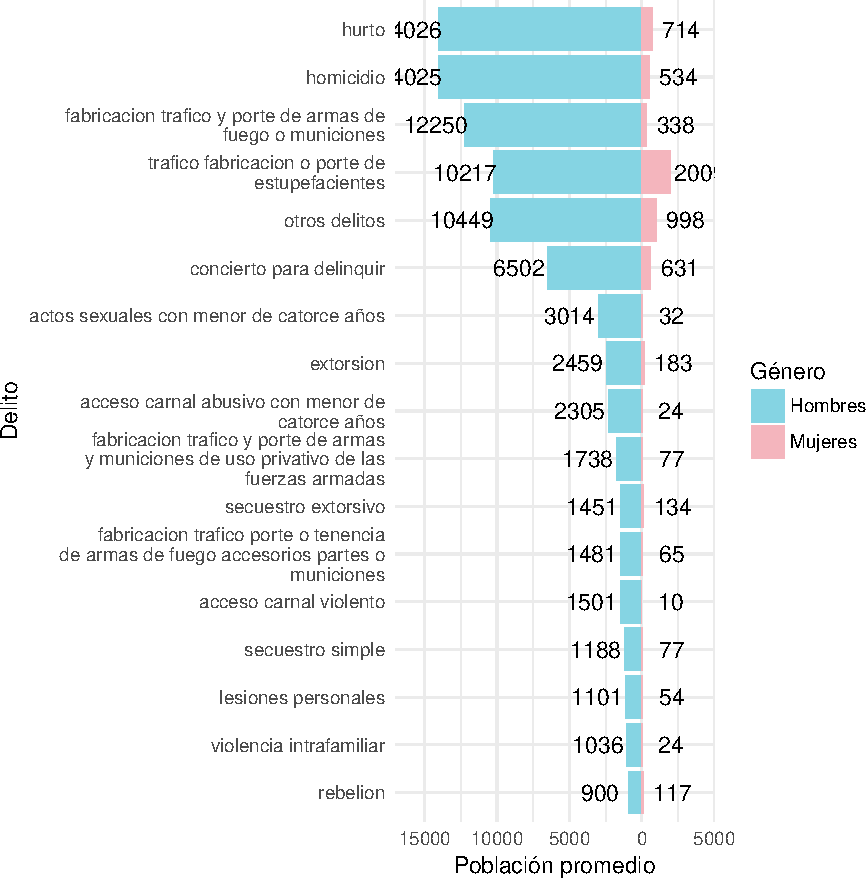
\includegraphics[width=0.7\linewidth]{delito-1.pdf}
	\caption{Poblaci�n carcelaria promedio por delito genero Octubre 2013-Diciembre 2016} {Fuente: INPEC} {Elaboraci�n propia}
	\label{fig:delito}
\end{figure}

\begin{figure}[H]
	\centering
	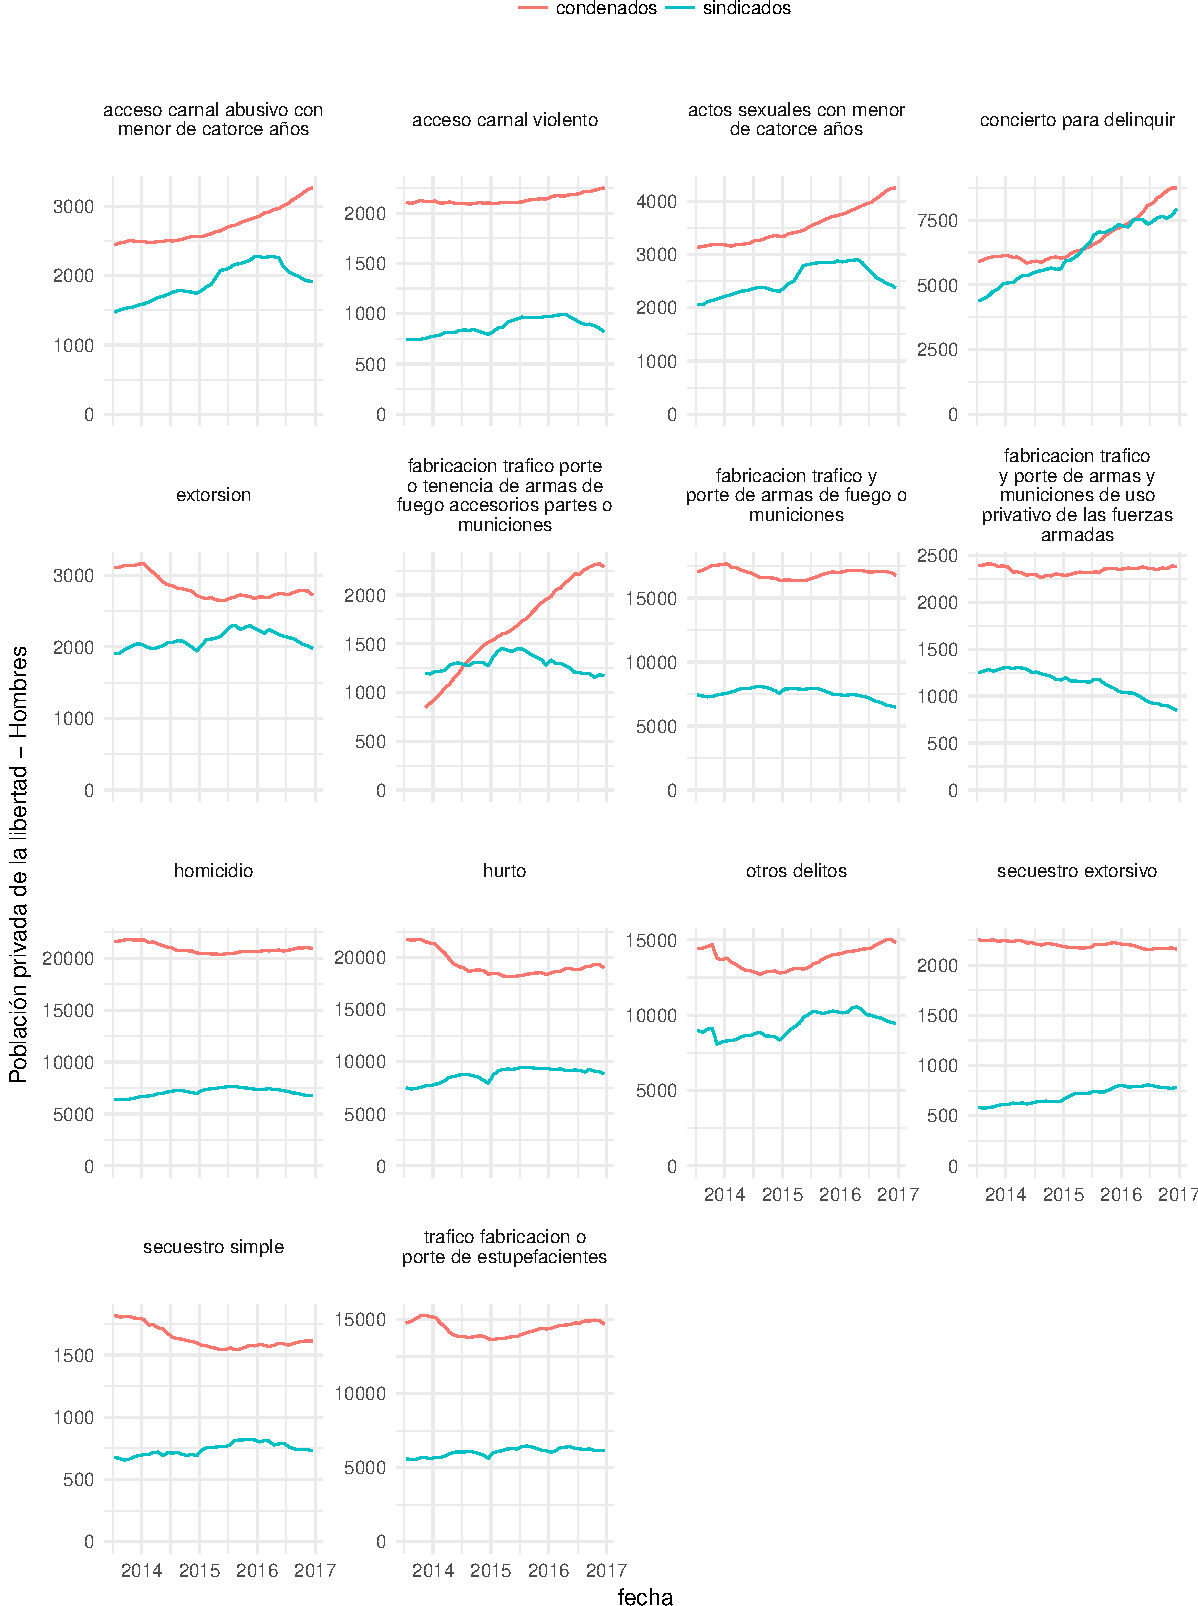
\includegraphics[width=1\linewidth]{delitoshombres-1.pdf}
	\caption{Evoluci�n de la poblaci�n carcelaria masculina, Octubre 2013-Diciembre 2016} {Fuente: INPEC} {Elaboraci�n propia}
	\label{fig:delitoshombres}
\end{figure}

\begin{figure}[H]
	\centering
	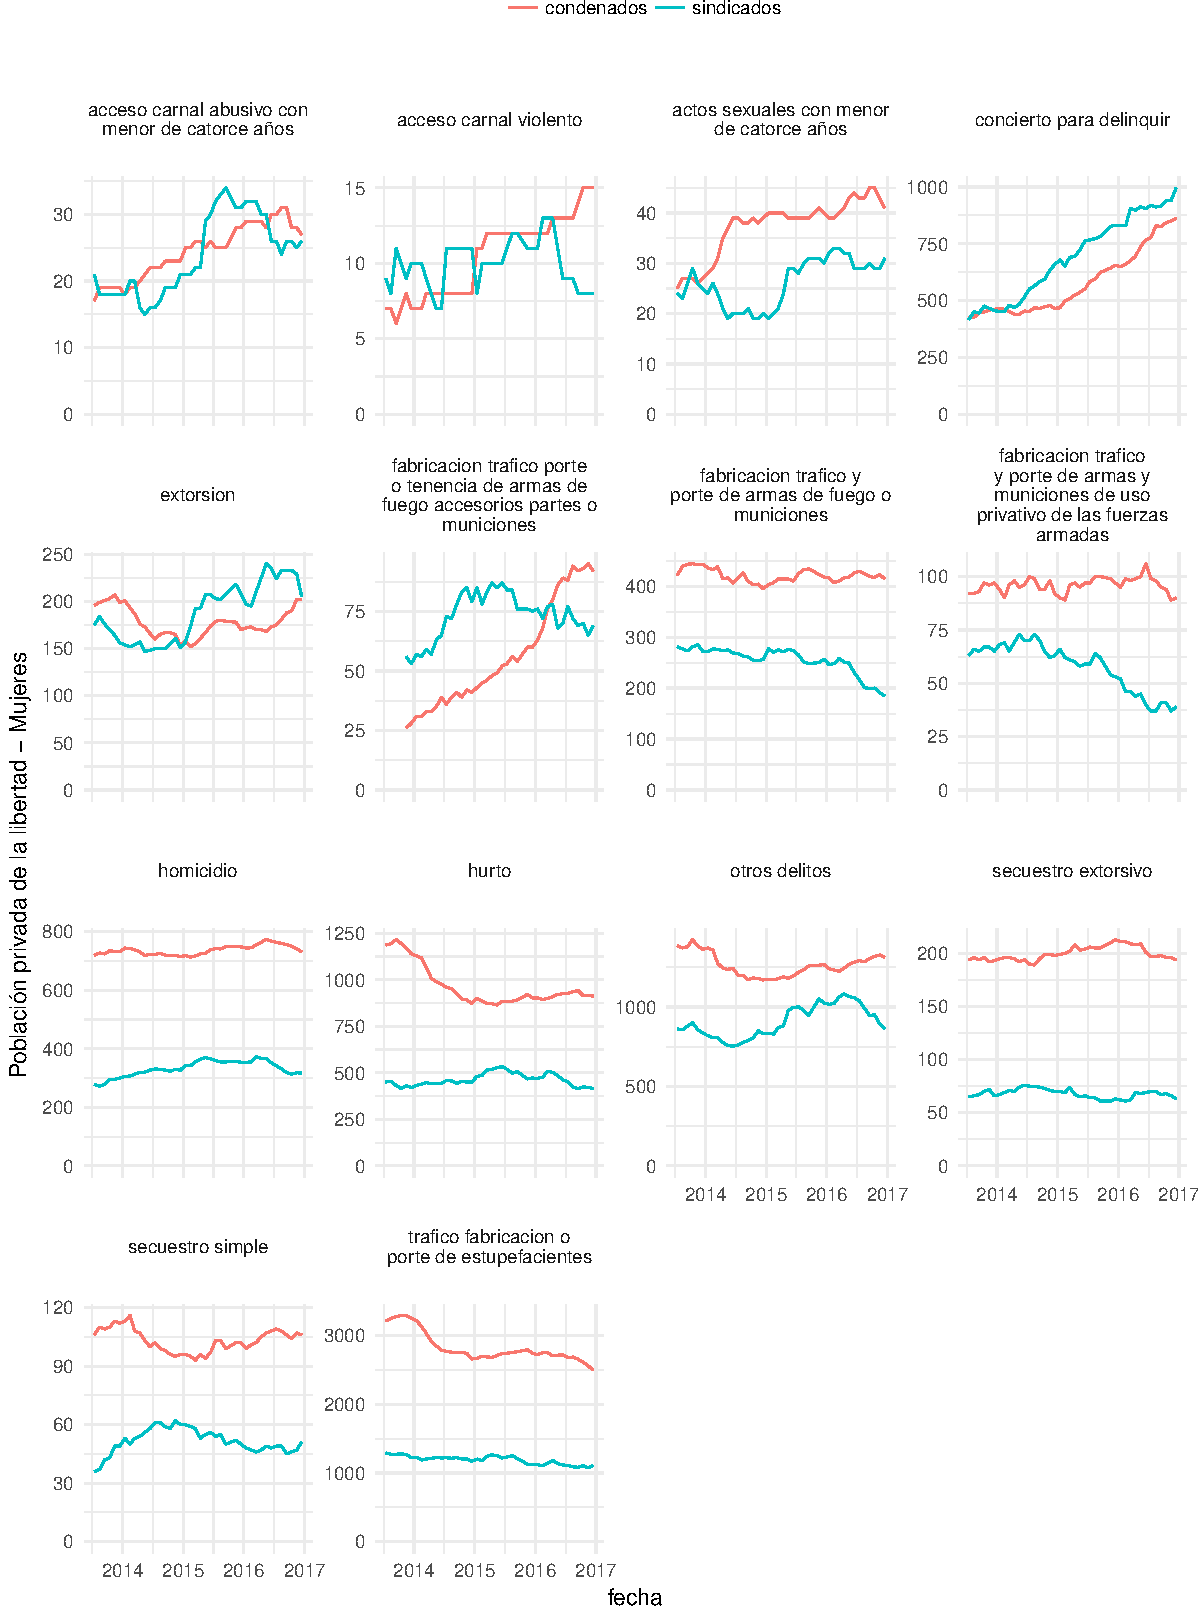
\includegraphics[width=1\linewidth]{delitosmujeres-1.pdf}
	\caption{Evoluci�n de la poblaci�n carcelaria femenina, Octubre 2013-Diciembre 2016} {Fuente: INPEC} {Elaboraci�n propia}
	\label{fig:delitosmujeres}
\end{figure}

\section{Selecci�n de Software}

Para mantener un �nico ambiente de desarrollo, nos enfocamos en los paquetes desarrollados en R, como los mencionados por Petris \cite{Petris2011}, Helske \cite{Helske2017} y Tusell \cite{Tusell2011}. Dentro de los paquetes analizados se encuentran  \textit{Kfas} por Helske(2017) \cite{Helske2017} y \textit{MARSS} de Holmes(2018) \cite{Holmes2018}. Se utiliza \textit{MARSS} por la simplicidad en la definici�n del modelo.

\section{Identificaci�n del modelo}

Holmes \& Ward \& Willis (2018) definen los modelos MARSS, Modelos auto-regresivos multivariados, de forma general como: 

\begin{equation}
x_{t}  B_{t}x_{t-1} +u_t +C_tc_t +G_tw_t \quad donde \quad w_t \sim MVN(0,Q_t)
\end{equation}

\begin{equation}
y_{t} = Z_{t}x_{t} +a_{t} +D_{t}d_{t} +H_{t}v_{t} \quad donde \quad v_t \sim MVN(0,R_t)
\end{equation}


\begin{equation}
x_1 \sim MVN(\pi,\Lambda)\, o \, x_0 \sim MVN(\pi,\Lambda)
\end{equation}

%%%%%%%%%%%%%%%%%%%%%%%%%%%%%%%%
PENDIENTE PONER SIGNIFICADO DE LAS ECUACIONES
%%%%%%%%%%%%%%%%%%%%%%%%%%%%%%%%

En este cap�tulo se usar� el modelo bivariado: 

\begin{equation}
\begin{bmatrix} X1_t  \\ X2_t \end{bmatrix} =
\begin{bmatrix}
b1 & 0 \\
b2 & b4 &
\end{bmatrix} 
\begin{bmatrix} X1_{t-1}  \\ X2_{t-1} \end{bmatrix} +
\begin{bmatrix} U1_t  \\ U2_t \end{bmatrix} , \begin{bmatrix} U1_t  \\ U2_t \end{bmatrix} \sim MVN(\begin{bmatrix} 0  \\ 0 \end{bmatrix},  \begin{bmatrix} q_{11}  &  q_{12} \\ q_{12} & 1_{22}\end{bmatrix})
\end{equation}

\begin{equation}
\begin{bmatrix} Y1_t  \\ Y2_t \end{bmatrix} =
\begin{bmatrix}
1 & 0 \\ 0 & 1
\end{bmatrix} 
\begin{bmatrix} X1_{t-1}  \\ X2_{t-1} \end{bmatrix} +
\begin{bmatrix} V1_t  \\ V2_t \end{bmatrix} , \begin{bmatrix} V1_t  \\ V2_t \end{bmatrix} \sim MVN(\begin{bmatrix} 0  \\ 0 \end{bmatrix},  \begin{bmatrix} 0 &  0 \\ 0 & 0 \end{bmatrix})
\label{equ:observado}
\end{equation}

Donde 

$X1_t$ = Poblaci�n sindicada en el periodo t

$X2_t$ = Poblaci�n condenada en el periodo t

$U_1t$ = Variaci�n mensual en la poblaci�n sindicada no asociada a la poblaci�n sindicada en el periodo anterior. 

$U_1t$ = Variaci�n mensual en la poblaci�n condenada no asociada a la poblaci�n sindicada, ni condenada en el periodo anterior. 

La ecuaci�n \ref{equ:observado} implica que el estado observado es id�ntico al estado real del sistema. Sin embargo, tratarlo como un modelo estado espacio permite trabajar los datos faltantes sin inconvenientes.

\section{Estimaci�n de par�metros}

La estimaci�n se realiza en series bivariadas por delito, g�nero. Se presenta en detalle procedimiento para la serie de hurto en hombres, en series adicionales se presentan resultados de la proyecci�n.

% latex table generated in R 3.4.4 by xtable 1.8-2 package
% Fri Jun  8 10:38:47 2018
\begin{table}[ht]
	\centering
	\begin{tabular}{rr}
		\hline
		Par�metro & estimado \\ 
		\hline
		b1 & 0.94 \\ 
		b2 & 0.07 \\ 
		b4 & 0.97 \\ 
		u1 & 557.98 \\ 
		u2 & -147.10 \\ 
		q11 & 33191.09 \\ 
		q12 & -5113.90 \\ 
		q22 & 33454.10 \\ 
		\hline
	\end{tabular}
	\caption{Par�metros estimados hurto hombres} {Fuente: INPEC} {Elaboraci�n propia}
	\label{tab:Estimadoshurtohombres}
\end{table}

\begin{figure}[H]
	\centering
	\includegraphics[width=0.7\linewidth]{estado_espacio_hurto-1.pdf}
	\caption{Poblaci�n sindicada y condenada por hurto, hombres} {Fuente: INPEC} {Elaboraci�n propia}
	\label{fig:estadoespacioinputa}
\end{figure}

\begin{figure}[H]
	\centering
	\includegraphics[width=0.7\linewidth]{estado_espacio_hurto-2.pdf}
	\caption{Poblaci�n carcelaria promedio por delito genero Octubre 2013-Diciembre 2016} {Fuente: INPEC} {Elaboraci�n propia}
	\label{fig:estadoespacioqqplot}
\end{figure}

\section{Proyecciones 2017 - 2020}

Se realiza proyecci�n de la poblaci�n media sindicada y condenada en la tabla 

% latex table generated in R 3.4.4 by xtable 1.8-2 package
% Fri Jun  8 11:27:07 2018
\begin{table}[H]
	\centering
	\begin{tabular}{rlrr}
		\hline
		& Periodo & Sindicados & Condenados \\ 
		\hline
		V1 & 2017-01-15 & 8866.00 & 18988.00 \\ 
		V2 & 2017-02-15 & 8887.00 & 18946.00 \\ 
		V3 & 2017-03-15 & 8907.00 & 18905.00 \\ 
		V4 & 2017-04-15 & 8926.00 & 18868.00 \\ 
		V5 & 2017-05-15 & 8944.00 & 18832.00 \\ 
		V6 & 2017-06-15 & 8960.00 & 18799.00 \\ 
		V7 & 2017-07-15 & 8976.00 & 18768.00 \\ 
		V8 & 2017-08-15 & 8991.00 & 18739.00 \\ 
		V9 & 2017-09-15 & 9004.00 & 18711.00 \\ 
		V10 & 2017-10-15 & 9017.00 & 18686.00 \\ 
		V11 & 2017-11-15 & 9029.00 & 18661.00 \\ 
		V12 & 2017-12-15 & 9041.00 & 18639.00 \\ 
		V13 & 2018-01-15 & 9052.00 & 18617.00 \\ 
		V14 & 2018-02-15 & 9062.00 & 18598.00 \\ 
		V15 & 2018-03-15 & 9071.00 & 18579.00 \\ 
		V16 & 2018-04-15 & 9080.00 & 18561.00 \\ 
		V17 & 2018-05-15 & 9088.00 & 18545.00 \\ 
		V18 & 2018-06-15 & 9096.00 & 18529.00 \\ 
		V19 & 2018-07-15 & 9104.00 & 18515.00 \\ 
		V20 & 2018-08-15 & 9111.00 & 18501.00 \\ 
		V21 & 2018-09-15 & 9117.00 & 18489.00 \\ 
		V22 & 2018-10-15 & 9123.00 & 18477.00 \\ 
		V23 & 2018-11-15 & 9129.00 & 18465.00 \\ 
		V24 & 2018-12-15 & 9134.00 & 18455.00 \\ 
		V25 & 2019-01-15 & 9140.00 & 18445.00 \\ 
		V26 & 2019-02-15 & 9144.00 & 18436.00 \\ 
		V27 & 2019-03-15 & 9149.00 & 18427.00 \\ 
		V28 & 2019-04-15 & 9153.00 & 18419.00 \\ 
		V29 & 2019-05-15 & 9157.00 & 18411.00 \\ 
		V30 & 2019-06-15 & 9161.00 & 18404.00 \\ 
		V31 & 2019-07-15 & 9164.00 & 18398.00 \\ 
		V32 & 2019-08-15 & 9167.00 & 18391.00 \\ 
		V33 & 2019-09-15 & 9171.00 & 18386.00 \\ 
		V34 & 2019-10-15 & 9173.00 & 18380.00 \\ 
		V35 & 2019-11-15 & 9176.00 & 18375.00 \\ 
		V36 & 2019-12-15 & 9179.00 & 18370.00 \\ 
		\hline
	\end{tabular}
	\caption{Proyecci�n a treinta y seis meses hurto hombres} {Fuente: INPEC} {Elaboraci�n propia}
	\label{tab:Estimadoshurtohombres}
\end{table}

%%%%%%%%%%%%%%%%%%%%%%%%%%%%%%%%%%
PENDIENTE REALIZAR PROYECCIONES DEL RESTO DE SERIES Y PRESENTAR CONSOLIDADO
%%%%%%%%%%%%%%%%%%%%%%%%%%%%%%%%%%
\section{Discusi�n}